\documentclass[11pt]{report}
\usepackage[italian]{babel}
\usepackage[utf8]{inputenc}
\usepackage[T1]{fontenc}
\usepackage[nomarginpar]{geometry}
\usepackage{graphicx}
\graphicspath{ {images/} }

\usepackage[pdftex,
			pdfauthor={Eugenio Severi, Stefano Belli},
			pdftitle={Progetto ASW - id3king-js},
			pdfsubject={Relazione progetto Applicazioni e Servizi Web},
			pdfkeywords={id3king id3king-js ASW},
			pdfproducer={Latex with hyperref},
			pdfcreator={pdflatex}]{hyperref}
\pagestyle{plain}

\begin{document}
\title{Progetto di Applicazioni e Servizi Web\\id3king-js}
\author{Eugenio Severi, Stefano Belli}
\date{A.A. 2016-2017}
\begin{titlepage}
	\maketitle
\end{titlepage}

\setcounter{chapter}{1}
\section{Introduzione}
L'escursionismo è un attività motoria nel quale viene percorso un certo tragitto nel territorio su percorsi tipicamente agevoli, a scopo ricreativo o di studio.
\\Essendo un attività a basso sforzo fisico e molto modulabile nella sua difficoltà, è una pratica molto diffusa nel mondo e nel nostro paese da persone di tutte le fasce d'età.\\
I percorsi solitamente utilizzati dagli escursionisti sono interamente mappati su apposite cartine topografiche e il loro stato di percorrenza viene mantenuto costantemente da alcuni enti preposti come il \textit{CAI} (Club Alpino Italiano).
\\Tuttavia, l'escursionismo richiede molta attenzione nella sua pianificazione, in quanto è facile sbagliare la stima della lunghezza del percorso o il suo dislivello.
\\Molti escursionisti "occasionali" si ritrovano, loro malgrado, a capire esattamente le difficoltà di un percorso soltanto una volta sul luogo, magari a metà dell'escursione.
\\\\Fortunatamente, alcuni gruppi di escursionisti amatoriali redigono e pubblicano della documentazione sulle escursioni da loro intraprese: il più famoso di essi nella zona emiliano-romagnola è \textit{id3king}.
\\Il sito del gruppo (www.id3king.it), infatti, viene aggiornato regolarmente, con nuove escursioni inserite spesso su base settimanale.
Per ogni escursione presente, è possibile scaricarne il tracciato GPS, la tabella dei toponimi e una sezione della cartina del percorso, oltre a molte altre informazioni.
\\Data la relativa difficoltà di trovare informazioni così dettagliate sui percorsi escursionistici e di una tale entità (allo stato attuale, il sito presenta oltre 890 escursioni documentate su un arco di diciotto anni!), è evidente che il lavoro di questo gruppo sia di enorme rilevanza per tutti gli appassionati di escursionismo.
\\Tuttavia, allo stato attuale, il sito del gruppo non consente di filtrare a piacimento le escursioni inserite, così come ordinarle secondo un altro criterio oltre a quello della data di inserimento; queste mancanze rendono piuttosto difficoltoso trovare rapidamente l'escursione adatta alle proprie esigenze.
\\\\A causa di queste mancanze, è nato il progetto \textit{id3king-js}: ottenuto il consenso da parte degli amministratori del sito si è deciso di progettare e sviluppare una web app che esegua lo scraping dell'originale e proponga i dati presenti in maniera maggiormente fruibile e funzionale, ad esempio permettendo una ricerca basata su parametri e la creazione di profili utente per memorizzare dati di interesse.
\\In particolare dovrà essere possibile filtrare e riordinare gli itinerari del sito per consentire una più veloce individuazione di un percorso in base a una certa esigenza.
Ad esempio, un utente alla ricerca di un percorso non troppo impegnativo potrebbe pensare di filtrare tutti gli itinerari con lunghezza e dislivello inferiori a un certo quantitativo, e magari posti nella zona del lago di Ridracoli (FC).
\\Le funzionalità offerte dall'applicazione possono essere riassunte con il diagramma dei casi d'uso in figura \ref{use_case_diagram}.
\begin{figure}
	\centering
	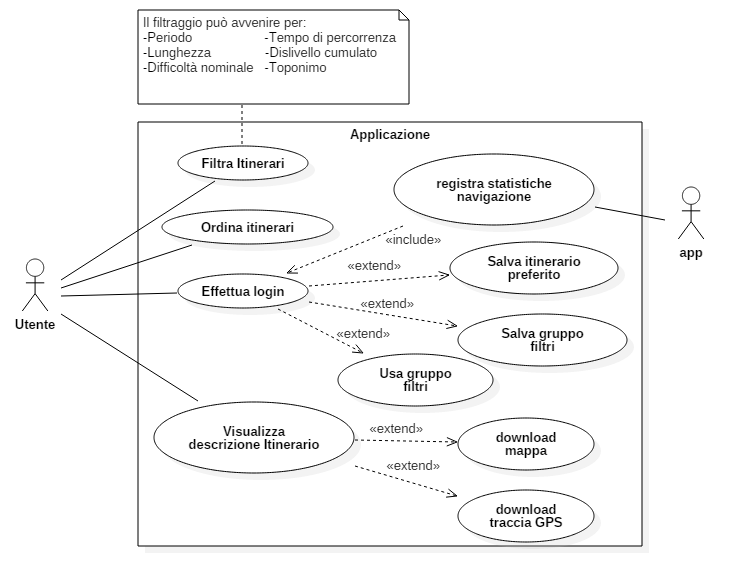
\includegraphics[scale=0.5]{use_case_diagram}
	\caption{Diagramma dei casi d'uso \label{use_case_diagram}}
\end{figure}
Il sistema dovrà rispettare requisiti di estensibilità, reattività, sicurezza e facilità d'uso per l'utente.

\pagebreak
\section{Architettura}
Per raggiungere gli obbiettivi preposti, sarà necessario realizzare un'opportuna architettura server, un back-end e un front-end in grado di gestire le sessioni utente e restituire gli itinerari presenti sul sito; pertanto, l'architettura del sistema è basata su una soluzione client-server.
\\Il server, inoltre, si occuperà di effettuare periodicamente lo scraping del sito: i dati estratti verranno riversati in un apposito database relazionale da cui si potrà attingere per ogni richiesta degli utenti.
\\Riepilogando, l'architettura sarà composta dai seguenti componenti:
\begin{itemize}
	\item un insieme di client che ottengono e utilizzano a piacimento i dati degli itinerari, attraverso un interfaccia web semplice e intuitiva;
	\item un server web che risponde alle esigenze dei client fornendo loro itinerari e altre funzionalità ad alto livello;
	\item un database relazionale in cui mantenere i dati degli utenti e gli itinerari ottenuti tramite scraping.
\end{itemize}
Adottando una architettura \textit{RESTful}, le comunicazioni I/O dell'applicazione sono completamente\textit{stateless}, consentendo di implementare facilmente un'architettura scalabile a livelli con nodi di commutazione intermedi.
\\Inoltre, essendo le comunicazioni basate su HTTP POST e GET, la portabilità dell'applicazione è totale in quanto universalmente compatibile.
\\In base ai requisiti precedentemente definiti, come framework di sviluppo si è valutato di usare \textit{Node.js}, che prevede l'utilizzo di tecnologie web sia client-side che server-side e consente di utilizzare un modello di comunicazione event-driven, particolarmente utile in un'applicazione di rete.
\\Il pattern \textit{MVC} (Model View Controller) è stato utilizzato per rendere più gestibili, modulari e riutilizzabili le singole componenti.
\\Ai fini di questo progetto si è scelto di utilizzare un unico server cloud di tipo \textit{IaaS} (Infrastructure as a Service), fornito da un provider, sul quale saranno installati tutti i servizi necessari al funzionamento dell'applicazione.
Sono tuttavia possibili configurazioni ridondanti, sia per il server web, sia per il DBMS, al fine di migliorare robustezza, affidabilità e tolleranza ai guasti.
% TODO: diagramma di deployment

\pagebreak
\section{Sicurezza}
Data la natura di rete dell'applicazione e poiché verranno trattati alcuni dati personali degli utenti (come ad esempio le password), è stato opportuno considerare la sicurezza già in fase di progettazione, onde evitare lacune successive difficili da individuare e rimuovere.
\begin{itemize}
	\item Tutte le comunicazioni di rete sono crittografate e autenticate con SSL/TLS per prevenire intercettazioni e attacchi \textit{man-in-the-middle}; cioè è stato reso possibile grazie alla grande flessibilità del framework Hapi, che consente di impostare semplicemente comunicazioni crittografate client-server.
	\\Pertanto, tutte le comunicazioni client-server avvengono tramite HTTPS e si possono ritenere quindi relativamente sicure.
	\item Tutte le credenziali degli utenti vengono memorizzate sotto forma di hash con \textit{salt}, grazie alla libreria per NodeJS \textit{bcrypt}.
	\\Tale libreria utilizza una funzione di hashing omonima che, a differenza delle più popolari \textit{SHA*}, adotta un approccio \textit{slow hash}, molto più adatto in questi contesti di sicurezza.
	%inserire bibliografia in "più adatta[1]" http://worldcomp-proceedings.com/proc/p2016/ICW3865.pdf
	\\Pertanto, considerando che le password rielaborate arrivano a sessanta caratteri, si può affermare che la sicurezza delle password salvate sul database sia più che resistente agli attuali metodi di cracking.
	\item Tutti gli input utente vengono validati per impedire lo sfruttamento di attacchi come \textit{SQL injection} e \textit{buffer overflow}, tramite la dalla libreria di interfacciamento col DB, \textit{mysql}. Inoltre, non sono consentite query SQL multiple per una sola richiesta.
	\item L'intero codice sorgente dell'applicazione è disponibile (e aperto a modifiche e miglioramenti) su \textit{Github}.
	\\Eventuali \textit{exploit} nel codice diventerebbero perciò trasparenti alla comunità e, pertanto, prontamente segnalati.
\end{itemize}
\pagebreak

\section{Back-end}
Il back-end è implementato in Javascript su NodeJS, utilizzando il framework \textit{Hapi}, nel rispetto del pattern MVC.
\\Un controller si occupa di interfacciarsi con i client, fungendo da mediatore con le funzioni più a basso livello, delegate ad apposite classi:
\begin{itemize}
	\item \textit{dbHandler}, che si occupa dell'interfacciamento con il database e fornisce intefacce ad alto livello per eseguire operazioni complesse;
	\item \textit{scraper}, che scansiona il sito "id3king.it" alla ricerca di nuove informazioni da normalizzare ed aggiungere al database.
	La normalizzazione è resa necessaria per l'inserimento nel database, in quanto sul sito originale i dati sono inseriti in HTML come stringhe semplici e quindi non normalizzati.
\end{itemize}
\subsection{Diagramma delle classi}
Nel diagramma delle classi è rappresentata la struttura del back-end.
%TODO: diagramma delle classi
\subsection{Diagramma di sequenza}
Nel diagramma di sequenza è esplicitato il funzionamento di una generica chiamata proveniente da un client che necessita di accedere ad informazioni presenti nel database.
%TODO: diagramma di sequenza
\subsection{Dati e database}
Il DBMS scelto per l'implementazione è \textit{MariaDB}.
\\La tabella principale è \textit{Percorso} che, insieme a \textit{Localita}, contiene i dati ottenuti tramite scraping.
Gli amministratori possono opzionalmente modificare manualmente questi dati qualora le informazioni riportate non fossero corrette: questo può accadere poiché i dati originali non sono normalizzati.
Di conseguenza, potrebbero occasionalmente presentarsi dati errati o mal formattati.
Anche per questo motivo, si è scelto di popolare il contenuto di queste tabelle in maniera non distruttiva durante lo scraping automatico.
\\Ogni volta che i dettagli di uno specifico percorso vengono visualizzati da un utente, il relativo contatore viene incrementato: in questo modo è possibile sapere quali sono gli itinerari più ricercati.
\\Altro fulcro di archiviazione dei dati è la tabella \textit{Utenti}, che memorizza i dati degli utenti del servizio e funge da identificatore nelle altre tabelle contenenti i dati degli utenti:
\begin{itemize}
	\item \textit{ItinerarioPreferito}, che consente ad ogni utente di salvare una serie di percorsi per poterli ritrovare facilmente in seguito;
	\item \textit{Login}, che memorizza per ogni sessione un token generato casualmente che scade dopo un periodo di tempo configurabile (utile per consentire sessioni multiple);
	\item \textit{Ricerca}, che consente ad ogni utente di memorizzare una serie di parametri di ricerca in modo da non doverli reimpostare ad ogni accesso.
\end{itemize}
Concludono lo schema le tabelle \textit{Difficolta} e \textit{Periodo}, necessarie affinché il database sia in terza forma normale.
\\In figura \ref{db_schema} è presente lo schema relazionale.
\begin{figure}
	\centering
	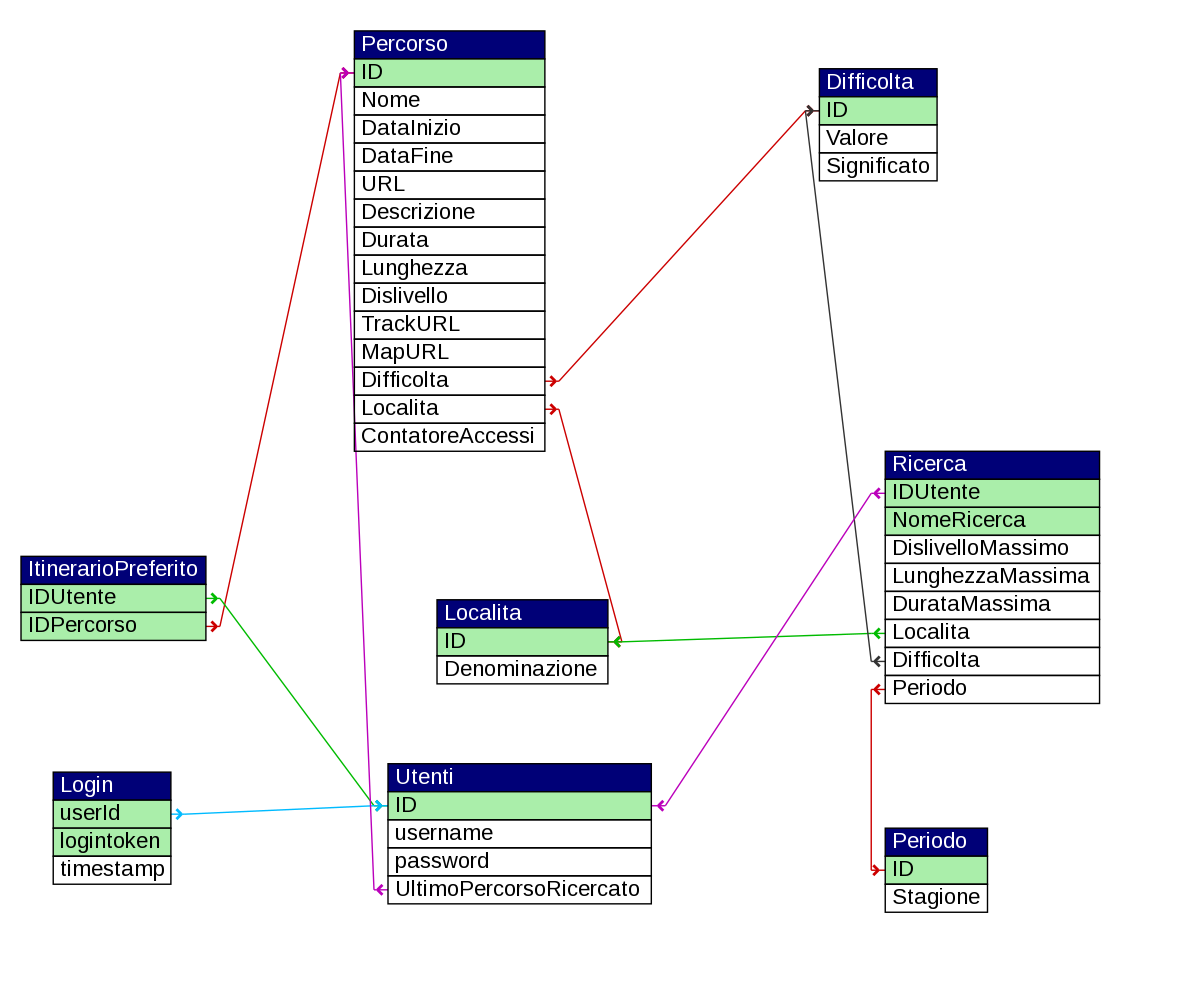
\includegraphics[scale=0.45]{DB_schema}
	\caption{Schema relazionale del database \label{db_schema}}
\end{figure}
\subsection{File di configurazione}
Tramite un file di configurazione (\textit{config.json}) è possibile personalizzare alcuni aspetti del funzionamento dell'applicazione:
\begin{itemize}
	\item la frequenza di scraping automatico (tramite \textit{cron});
	\item i parametri di connessione al DBMS;
	\item la porta su cui il server web deve restare in ascolto;
	\item i requisiti di sicurezza minimi per le credenziali degli utenti;
	\item i file del certificato e della chiave privata per SSL/TLS.
\end{itemize}

\section{Front-end}
%TODO: Angular in generale, pattern MVC (e altri?), descrizione interfaccia grafica (spiegazione funzioni principali con qualche screenshot).

\section{Conclusioni}


\end{document}
\endinput
